\documentclass[10pt,a4paper]{amsart}
\usepackage[margin=19mm]{geometry}
\usepackage{amsmath,amssymb,mathtools}
\usepackage[scr=rsfs,cal=euler]{mathalfa}
\usepackage{xfrac}
\usepackage[unicode,hidelinks,bookmarks=false]{hyperref}
\newcommand{\ie}{i.e.\ }
\newcommand{\cf}{cf.\ }
\newcommand{\resp}{respectively\ }
\newcommand{\Subsection}{\subsection}
\providecommand{\nobreakdash}{\nobreak\hbox{-}}
\setlength{\emergencystretch}{2em}
\multlinegap0pt
\usepackage{tikz}
\usetikzlibrary{arrows.meta}
\newtheorem{theorem}{Theorem}
\newtheorem{lemma}[theorem]{Lemma}
\hypersetup{pdftitle={Four collinear points or six visible points},
pdfsubject={A short proof that N(4,6) is at most 880}}
\begin{document}
\title[Four collinear points or six visible points]{Four collinear points or six visible points}
\author{Stijn Cambie}
\date{}
\maketitle
\noindent\emph{Source and licence.} Four collinear points or six visible points. Version arXiv:2609.21035v1 (CC BY 4.0). This material is distributed under the Creative Commons Attribution 4.0 International licence, http://creativecommons.org/licenses/by/4.0/, as recorded in the arXiv OAI licence metadata for this exact version and shown on the abstract page https://arxiv.org/abs/2609.21035v1. Full rights notice: licenses/arxiv-2609.21035-CC-BY-4.0.txt.\par\smallskip
\noindent\textit{Editorial scope.} Counted unit: the original \texttt{lemma} environment \texttt{graph} at source lines 78--84 together with its complete proof at lines 85--118; the delivered document keeps source lines 72--152 so that every referenced label and every citation resolves inside it. Native editable source is the paper's own concatenated TeX; the AMS wrapper is editorial formatting only. No publisher class, upstream script or unrelated artwork is redistributed.
\section{Proof}

For a graph $H$, write $e(H)$ for its number of edges and $N_H(v)$ for
the set of neighbors of a vertex $v$.



\begin{lemma}\label{graph}
If a $K_6$-free graph $H$ on $r\ge1$ vertices requires at least $q$ vertex deletions
to become $5$-colorable, where $0\le q\le r$, then
\[
             e(H)\le\frac{2r^2}{5}-\frac{q(r-q)}{10}.
\]
\end{lemma}

\begin{proof}
We start building a maximal clique vertex by vertex. Set $R_1=V(H)$.
For each $i$ with $R_i\ne\varnothing$, choose $v_i\in R_i$ of largest
degree in the original graph $H$, and put
$R_{i+1}=R_i\cap N_H(v_i)$.
Stop when $R_{k+1}=\varnothing$. Each chosen vertex is adjacent to all
earlier choices, and the stopping condition makes
$\{v_1,\ldots,v_k\}$ a maximal clique; see Figure~\ref{greedy}
(cf.~\cite[Section~2]{BN}).

Put $A_i=R_i\setminus R_{i+1}$. Thus $A_i$ consists of the vertices
whose first nonneighbor in the sequence is $v_i$, counting $v_i$ itself
as a nonneighbor. The sets $A_i$ partition $V(H)$.
Let $a_i=|A_i|$, $d_i=d_H(v_i)$, and
$\varepsilon_i=r-a_i-d_i\ge0$.
Each vertex of $A_i$ was available when $v_i$ was chosen, so
\[
       2e(H)\le\sum_i a_i d_i
       =r^2-\sum_i(a_i^2+a_i\varepsilon_i).
\]
If $k\le4$, Cauchy's inequality gives $e(H)\le3r^2/8$, which suffices
since $q(r-q)\le r^2/4$. Thus assume $k=5$.
Deleting the vertices missing two or more clique vertices leaves five
independent sets: an edge between two vertices missing only $v_i$ would
complete a $K_6$ with the other four clique vertices. Since
$\sum_i\varepsilon_i$ counts all misses beyond the first, it is at least
$q$. Choose $0\le x_i\le\varepsilon_i$ with $\sum_i x_i=q$. Then by Cauchy-Schwarz again
\[
 \sum_i(a_i^2+a_i\varepsilon_i)
 \ge\sum_i(a_i+x_i/2)^2-\frac14\sum_i x_i^2
 \ge\frac{(r+q/2)^2}{5}-\frac{q^2}{4}
 =\frac{r^2+q(r-q)}5.
\]
\end{proof}


\begin{figure}[htbp]
\centering
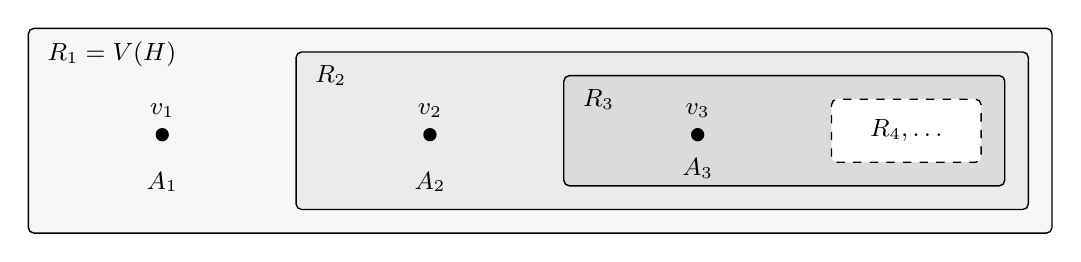
\begin{tikzpicture}[x=1cm,y=1cm,font=\small,
  region/.style={draw,rounded corners=2pt,line width=.5pt},
  point/.style={circle,fill=black,inner sep=1.7pt}]
  \path[region,fill=black!3] (0,0) rectangle (13,2.6);
  \path[region,fill=black!8] (3.4,.3) rectangle (12.7,2.3);
  \path[region,fill=black!14] (6.8,.6) rectangle (12.4,2.0);
  \path[region,dashed,fill=white] (10.2,.9) rectangle (12.1,1.7);
  \node[anchor=north west] at (.12,2.55) {$R_1=V(H)$};
  \node[anchor=north west] at (3.52,2.25) {$R_2$};
  \node[anchor=north west] at (6.92,1.95) {$R_3$};
  \node at (11.15,1.3) {$R_4,\ldots$};
  \node[point,label=above:$v_1$] at (1.7,1.25) {};
  \node[point,label=above:$v_2$] at (5.1,1.25) {};
  \node[point,label=above:$v_3$] at (8.5,1.25) {};
  \node at (1.7,.65) {$A_1$};
  \node at (5.1,.65) {$A_2$};
  \node at (8.5,.82) {$A_3$};
  % \draw[-{Stealth[length=4pt]}] (1.7,-.42) --
  %   node[below] {$\cap N_H(v_1)$} (5.1,-.42);
  % \draw[-{Stealth[length=4pt]}] (5.1,-.42) --
  %   node[below] {$\cap N_H(v_2)$} (8.5,-.42);
  % \draw[-{Stealth[length=4pt]}] (8.5,-.42) --
  %   node[below] {$\cap N_H(v_3)$} (11.9,-.42);
\end{tikzpicture}
\caption{Building a single clique. Choose $v_i$ from $R_i$ by comparing
  degrees in $H$, then keep only its neighbors as candidates for the next
  choice. The discarded part $A_i=R_i\setminus R_{i+1}$ includes $v_i$.
  The regions show sets of vertices, not their positions in the plane.}
\label{greedy}
\end{figure}


\begin{thebibliography}{99}
\bibitem[BN]{BN} B.~Bollob\'as and V.~Nikiforov, \emph{\href{https://doi.org/10.37236/1988}{The sum of degrees in cliques}}, Electron. J. Combin. \textbf{12} (2005), Note~N21.
\end{thebibliography}
\end{document}
